\documentclass[11pt,a4paper]{article}

\usepackage[T1]{fontenc}
\usepackage[utf8]{inputenc}
\usepackage{lmodern}
\usepackage[a4paper,margin=1in]{geometry}
\usepackage{amsmath,amssymb}
\usepackage{booktabs}
\usepackage{graphicx}
\usepackage{subcaption}
\usepackage{float}
\usepackage{hyperref}
\usepackage{enumitem}

\hypersetup{
  colorlinks=true,
  linkcolor=blue,
  citecolor=blue,
  urlcolor=blue
}

\title{Baseline Toy VELO Reconstruction Report\\\large Derived from \texttt{baseline.ipynb}}
\author{Quantum Track Reconstruction}
\date{\today}

\begin{document}
\maketitle

\begin{abstract}
This report documents the workflow and observed outputs in
\texttt{baseline.ipynb} in \texttt{Toy\_Characterisation}. The notebook establishes a
clean baseline for toy VELO track reconstruction, validates reconstruction
quality on single and multi-event samples, and studies pairwise segment-angle
separation between true and false combinations.
\end{abstract}

\section{Objective}
The baseline notebook is organized into four tasks:
\begin{enumerate}[leftmargin=1.5em]
  \item Build detector geometry and event-generation helpers.
  \item Reconstruct a clean 3-track event with a Hamiltonian solver and verify
  truth matching.
  \item Run a 10-event mixed-occupancy check and summarise efficiency/ghost
  behaviour.
  \item Measure true-vs-false pairwise segment-angle distributions, including
  a large-sample study (100 events \(\times\) 50 tracks).
\end{enumerate}

\section{Setup and Definitions}
\subsection{Geometry and Event Generation}
The baseline geometry and generation settings are:
\begin{itemize}[leftmargin=1.5em]
  \item 5 modules with positions
  \(z = [100,133,166,199,232]~\mathrm{mm}\) (\(\Delta z=33~\mathrm{mm}\)).
  \item Module half-widths \(l_x=l_y=50~\mathrm{mm}\).
  \item Primary-vertex and track generation via
  \texttt{StateEventGenerator}.
\end{itemize}

\subsection{Acceptance Scale}
The segment-angle acceptance threshold is computed as
\begin{equation}
\varepsilon = s\sqrt{2\theta_s^2 + 12\theta_r^2 + 2\theta_{\min}^2},
\end{equation}
with
\begin{equation}
\theta_s = \sigma_{\mathrm{scatt}},
\qquad
\theta_r = \arctan\left(\frac{\sigma_{\mathrm{res}}}{\Delta z}\right),
\end{equation}
and scale factor \(s=3\) in this notebook.

For the clean baseline:
\begin{itemize}[leftmargin=1.5em]
  \item \(\sigma_{\mathrm{res}} = 0\),
  \item \(\sigma_{\mathrm{scatt}} = 10^{-3}~\mathrm{rad}\),
  \item \(\Delta z = 33~\mathrm{mm}\),
\end{itemize}
which yields
\begin{equation}
\varepsilon = 0.004243~\mathrm{rad} = 4.243~\mathrm{mrad}.
\end{equation}

\section{Hamiltonian Reconstruction Baseline}
The clean event contains 3 truth tracks and 15 hits (5 hits per track).
Hamiltonian settings are
\(\gamma=1.5\), \(\delta=1.0\), and \(\varepsilon\) above.

The notebook uses
\begin{equation}
x_{\mathrm{baseline}} = \frac{\delta}{\delta+\gamma} = 0.4,
\qquad
x_{\mathrm{thr}} = \frac{1 + x_{\mathrm{baseline}}}{2} = 0.7.
\end{equation}

Observed solver output:
\begin{itemize}[leftmargin=1.5em]
  \item Number of segments: 36.
  \item Hamiltonian matrix: \(36\times 36\), \(\mathrm{nnz}=54\).
  \item Active above threshold: 12/36.
  \item Activation range: \([0.4000, 1.2727]\).
\end{itemize}

Reconstruction returns 3 tracks, each with 5 hits.

\begin{figure}[H]
  \centering
  \begin{subfigure}[b]{0.48\textwidth}
    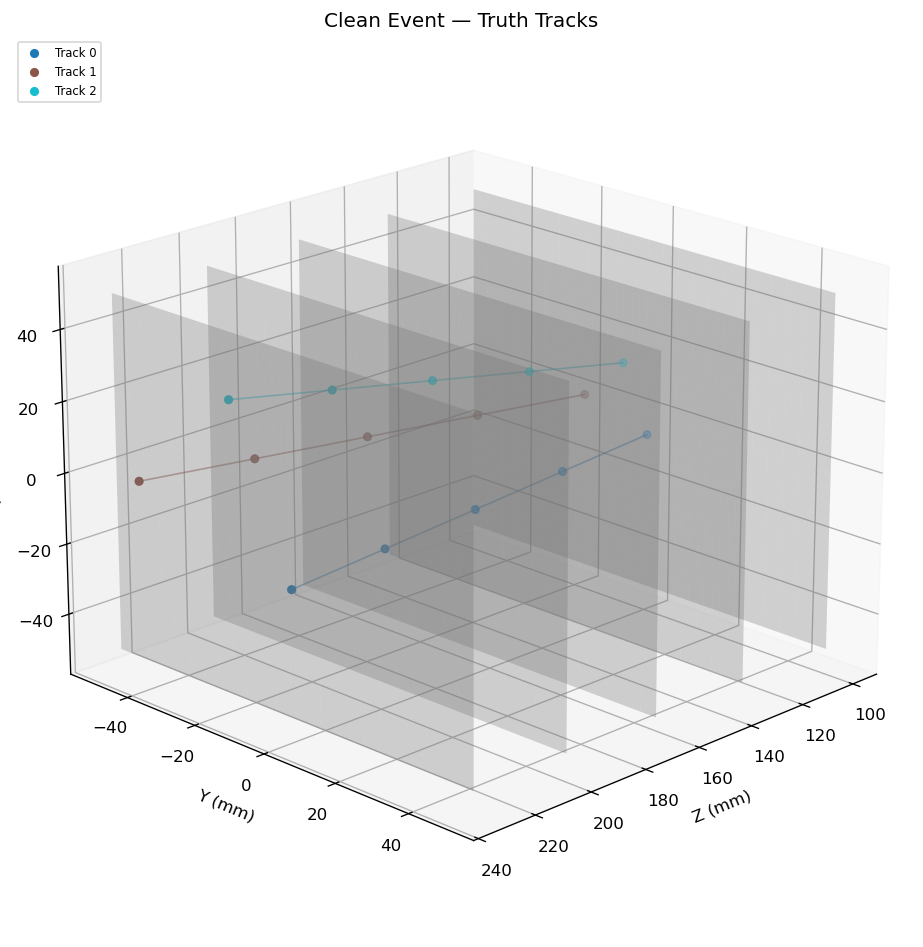
\includegraphics[width=\linewidth]{baseline_fig1_truth_3d.png}
    \caption{3-D truth event display (3 tracks).}
  \end{subfigure}\hfill
  \begin{subfigure}[b]{0.48\textwidth}
    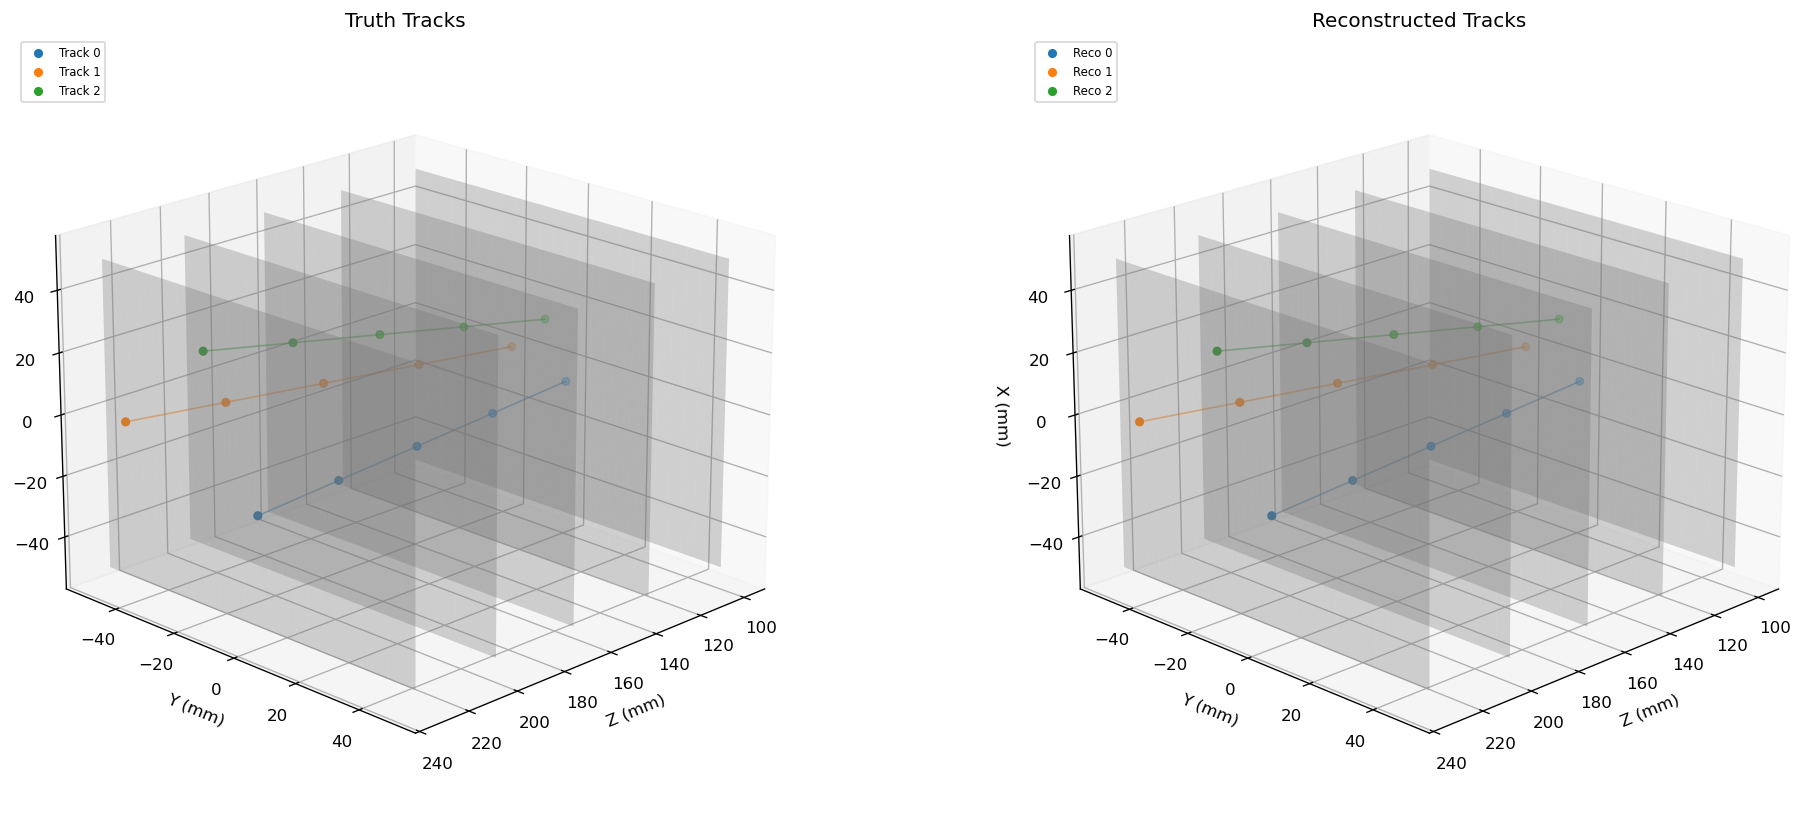
\includegraphics[width=\linewidth]{baseline_fig2_reco_truth_clean.png}
    \caption{Reconstructed vs.\ truth tracks.}
  \end{subfigure}
  \caption{Clean 3-track event. Left: truth geometry. Right: reconstructed overlay.}
  \label{fig:clean_event}
\end{figure}

\section{Clean-Event Validation}
Using \texttt{EventValidator} with \texttt{purity\_min=0.7}, all three truth
tracks are recovered as primary matches with purity and hit efficiency equal to
1.0.

\begin{table}[H]
\centering
\caption{Clean-event summary metrics.}
\begin{tabular}{lr}
\toprule
Metric & Value \\
\midrule
Efficiency & 1.0 \\
Ghost rate & 0.0 \\
Clone fraction & 0.0 \\
Mean purity & 1.0 \\
Hit efficiency & 1.0 \\
Matched / reconstructible & 3 / 3 \\
\bottomrule
\end{tabular}
\end{table}

For consecutive-segment pair angles on the clean event:
\begin{itemize}[leftmargin=1.5em]
  \item True pairs: 9, mean angle \(0.000000~\mathrm{rad}\).
  \item Reconstructed pairs: 9, mean angle \(0.000000~\mathrm{rad}\).
  \item Reference threshold: \(\varepsilon=0.004243~\mathrm{rad}\).
\end{itemize}

\begin{figure}[H]
  \centering
  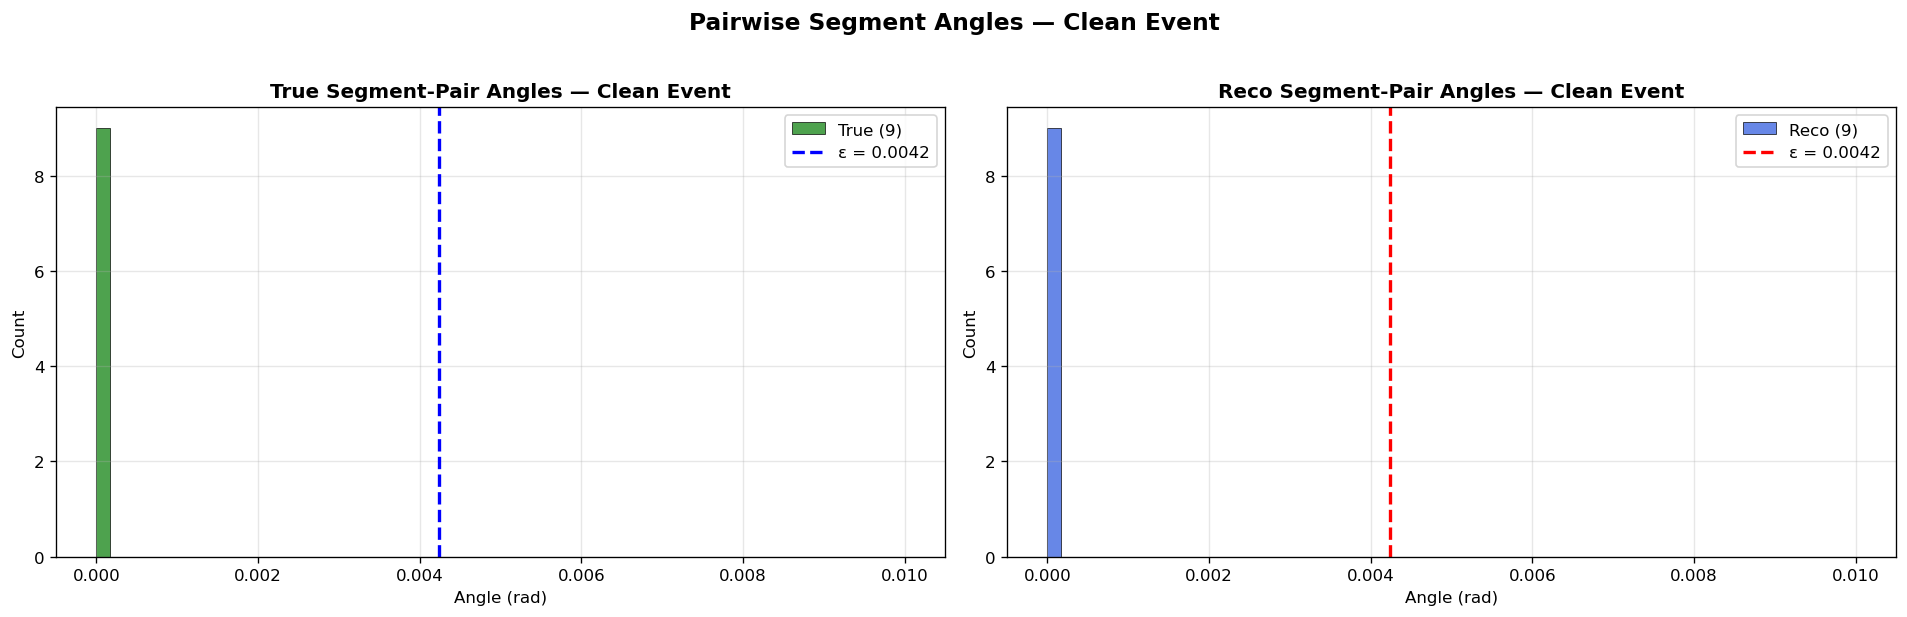
\includegraphics[width=0.95\textwidth]{baseline_fig3_seg_angles_clean.png}
  \caption{Pairwise segment-pair angles on the clean 3-track event.
    Left: true pairs (green). Right: reconstructed pairs (blue).
    All angles lie at exactly zero because the straight-line toy tracks have
    no multiple scattering.}
  \label{fig:seg_angles_clean}
\end{figure}

\section{10-Event Mixed-Occupancy Study}
Track-count schedule:
\([2,3,4,5,6,3,4,5,2,4]\).

\begin{table}[H]
\centering
\caption{Per-event baseline summary from notebook output.}
\begin{tabular}{rrrrrrr}
\toprule
Event & True & Reco & Eff & Ghost & TrueSeg & RecoSeg \\
\midrule
0 & 2 & 2 & 1.000 & 0.000 & 8 & 8 \\
1 & 3 & 3 & 1.000 & 0.000 & 12 & 12 \\
2 & 4 & 4 & 1.000 & 0.000 & 16 & 16 \\
3 & 5 & 5 & 1.000 & 0.000 & 20 & 20 \\
4 & 6 & 2 & 0.333 & 0.000 & 16 & 8 \\
5 & 3 & 3 & 1.000 & 0.000 & 12 & 12 \\
6 & 4 & 3 & 0.500 & 0.333 & 16 & 17 \\
7 & 5 & 5 & 1.000 & 0.000 & 20 & 20 \\
8 & 2 & 2 & 1.000 & 0.000 & 8 & 8 \\
9 & 4 & 4 & 1.000 & 0.000 & 16 & 16 \\
\bottomrule
\end{tabular}
\end{table}

Aggregate over the 10 events:
\begin{itemize}[leftmargin=1.5em]
  \item Mean efficiency: \(0.883\).
  \item Mean ghost rate: \(0.033\).
  \item Most events are perfectly reconstructed; notable degradation appears in
  events 4 and 6.
\end{itemize}

\section{Pairwise Segment-Angle Separation}
Angles are computed between segment pairs sharing a middle hit:
\begin{equation}
\alpha = \arccos\left(\frac{\mathbf{v}_1 \cdot \mathbf{v}_2}{\|\mathbf{v}_1\|\,\|\mathbf{v}_2\|}\right),
\end{equation}
where \(\mathbf{v}_1\) and \(\mathbf{v}_2\) are incoming/outgoing segment
vectors. A pair is labeled true only if all three hits are on the same truth
track.

Combined over the 10-event sample:
\begin{itemize}[leftmargin=1.5em]
  \item 106 true pairs,
  \item 1,742 false pairs.
\end{itemize}

\begin{figure}[H]
  \centering
  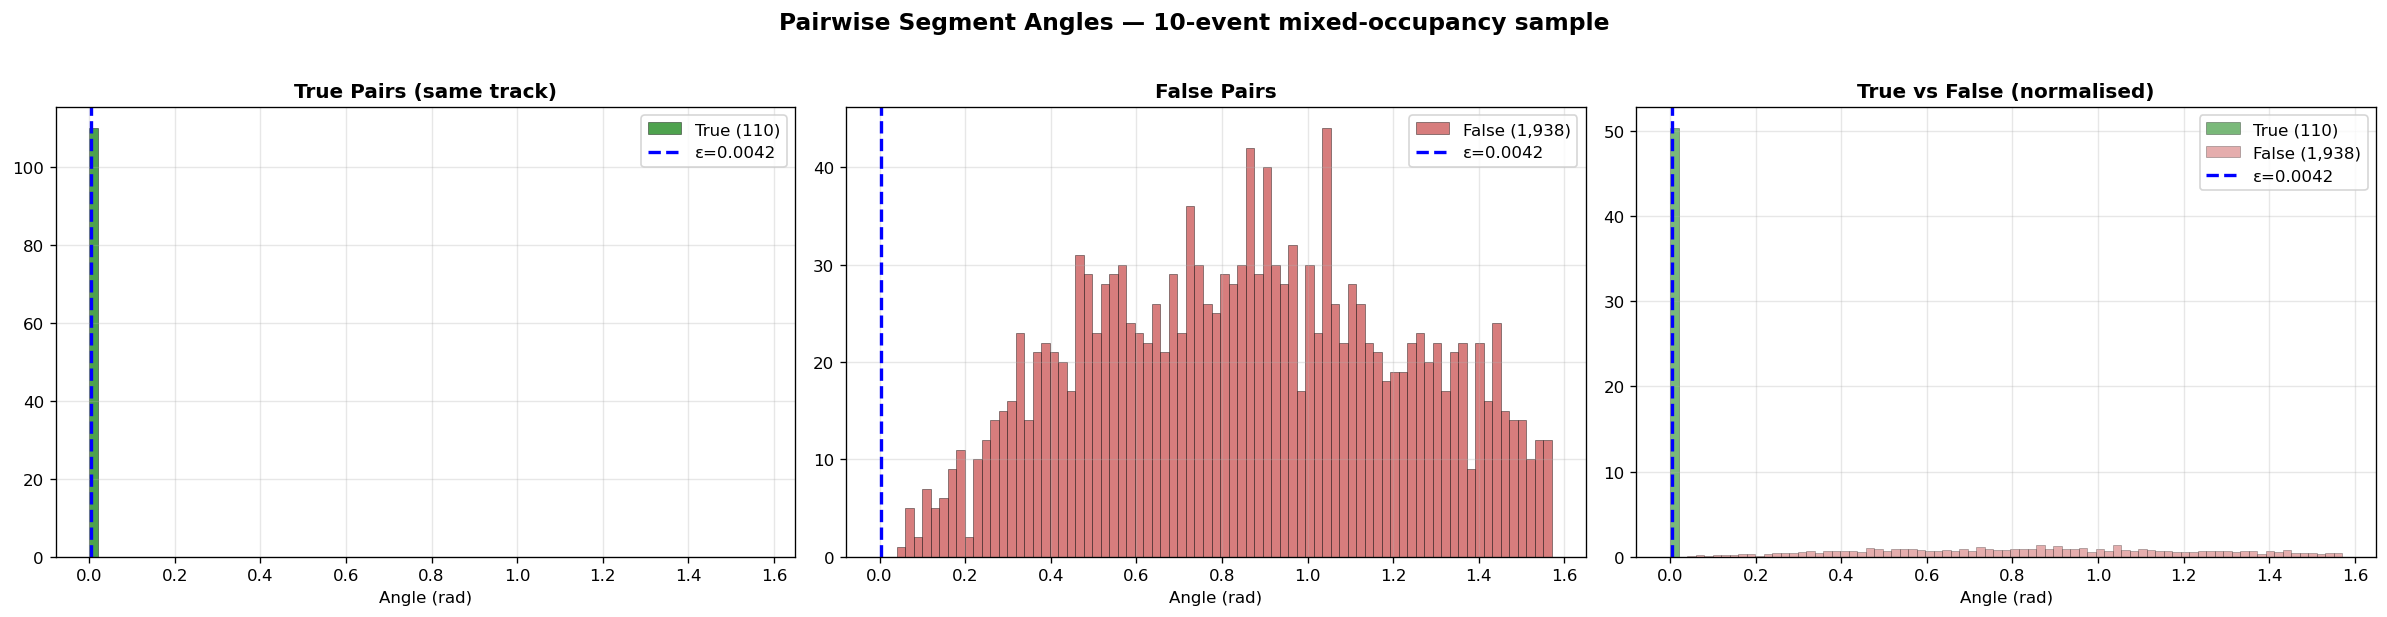
\includegraphics[width=0.97\textwidth]{baseline_fig4_seg_angles_10events.png}
  \caption{Pairwise segment-pair angles aggregated over the 10-event
    mixed-occupancy sample.
    Left: true pairs; centre: false pairs; right: normalised overlay.
    True pairs cluster near zero; false pairs are broadly distributed,
    confirming the threshold \(\varepsilon\) cleanly separates the two classes.}
  \label{fig:seg_angles_10events}
\end{figure}

Large-sample study (20 events \(\times\) 50 tracks):
\begin{itemize}[leftmargin=1.5em]
  \item 2,975 true segment pairs,
  \item 7,430,425 false segment pairs.
\end{itemize}

\begin{figure}[H]
  \centering
  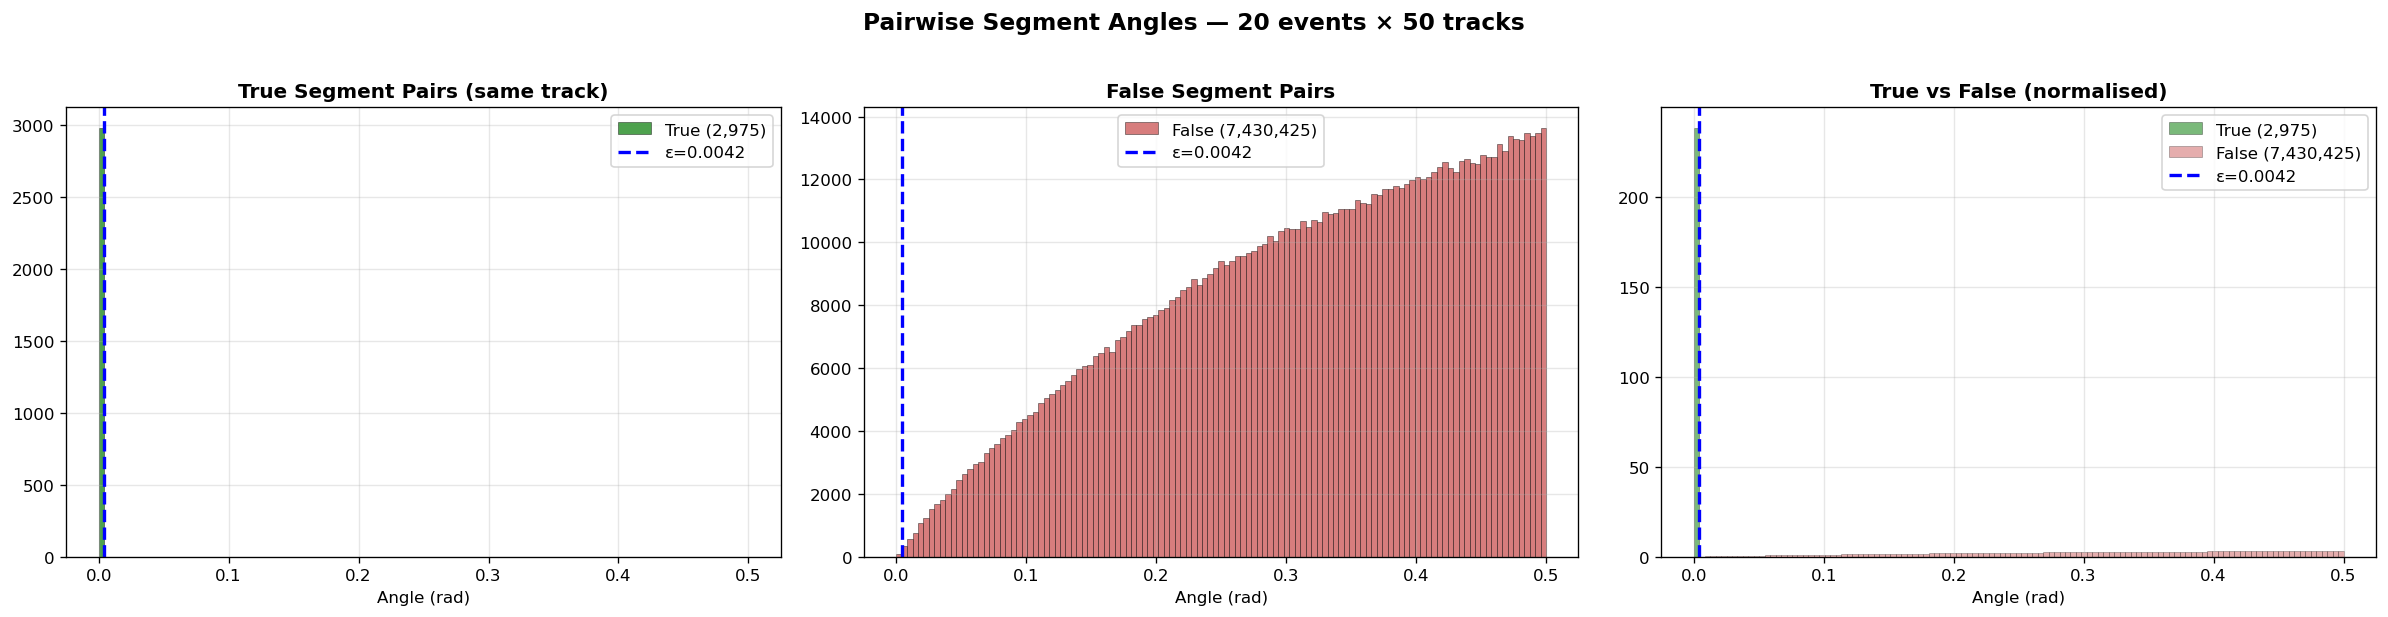
\includegraphics[width=0.97\textwidth]{baseline_fig5_seg_angles_large.png}
  \caption{Pairwise segment-pair angles for the large-sample run
    (20 events \(\times\) 50 tracks).
    The true-pair peak at zero and the broad false-pair distribution
    are consistent with the 10-event results, confirming stability
    at higher occupancy.}
  \label{fig:seg_angles_large}
\end{figure}

This large imbalance is expected combinatorially and motivates threshold-based
filtering in downstream reconstruction logic.

\section{Conclusion}
The baseline notebook demonstrates that the Hamiltonian-based reconstruction is
exact on the clean event and robust for most moderate-occupancy events. The
angle-distribution studies provide the intended separation context for true vs
false segment-pair combinations, and the 100\(\times\)50 run establishes a
high-statistics baseline for future tuning and comparisons.

\end{document}